% !TeX root =../../main.tex

\chapter{\mtfuzz: Multi-threading Aware Fuzzing} \label{ch:mtfuzz}

\section{Introduction}\label{sec:mtfuzz_intro}

\begin{figure}
\begin{center}
	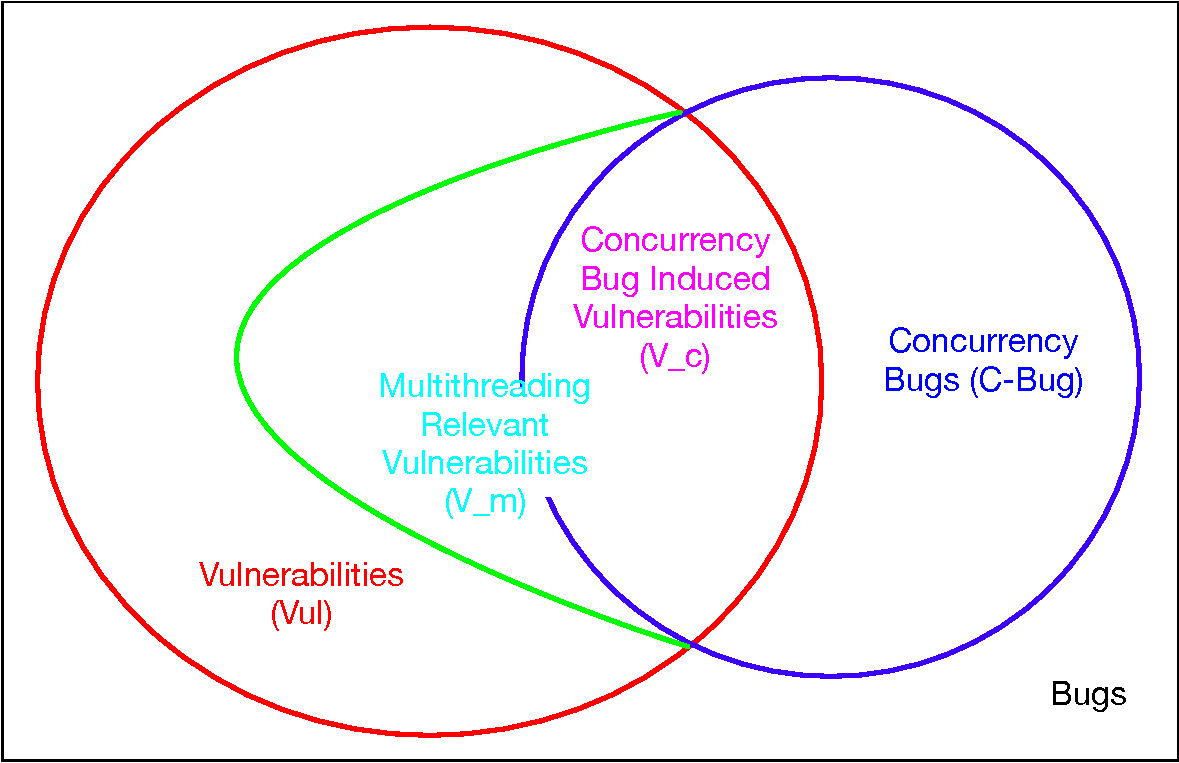
\includegraphics[width=0.5\textwidth]{res/venn}
	\caption{Venn Diagram of the Concurrency Relevant Vulnerabilities}
	\label{fig:venn_con_vul}
\end{center}	
\end{figure}

Multithreading as a popular programming paradigm is an effective way of utilizing multi-core computation resources in modern processors. Meanwhile, the \emph{non-deterministic} behaviors caused by thread-interleavings also pose substantial challenges to vulnerability or bug detection in multithreaded programs~\cite{mtbugs_survey}. On one hand, the interleavings across threads inherently introduce multiple subtle concurrency bugs, e.g., data races, atomic violations, and deadlocks. These bugs can cause undefined program behaviors and sometimes can induce vulnerabilities such as use-after-free (CVE-2016-1972, CVE-2018-5873) and heap-buffer-overflow (CVE-2017-8244), denial-of-service (CVE-2018-0381). On the other hand, as multithreaded programs may accept some inputs, some bugs or vulnerabilities may be difficult or impossible to be triggered with limited seed inputs, regardless of whether such bugs are caused by concurrency bugs. 



\setlength{\textfloatsep}{0.1cm} 
\begin{algorithm}[t]
 \small
\SetKwInOut{Input}{input}
	\SetKwInOut{Output}{output}
	\Input{Program \ProgO, Initial input test files \Seeds}
	\Output{Final test files \FinalSeeds, vulnerable test files \CrashSeeds}
	\Prog = instrument(\ProgO) \tcp*{static instrumentation}
	$\CrashSeeds \leftarrow~\emptyset$, $\FinalSeeds \leftarrow~\Seeds$\; 
	\While {True} {
		t = next\_seed(\FinalSeeds) \tcp*{seed selection}
		\mutChance = get\_mutation\_chance(t) \tcp*{seed scheduling} \label{line:algo:energy}
		\For {$i\in~1\ldots \mutChance$} {
			t' = mutated\_input(t)  \tcp*{seed mutation}
			res = run(\Prog, t', \Ncal)\tcp*{calibration execution}
			\uIf {is\_crash(res)}{\label{line:algo:triage_start}
				$\CrashSeeds = \CrashSeeds\cup\{t'\}$ \tcp*{report vulnerable seeds}
			}\ElseIf {cov\_new\_trace(t', res)} {\label{line:algo:new_cov}
				$\FinalSeeds = \FinalSeeds\cup\{t'\}$ \tcp*{save "good" seeds} \label{line:algo:triage_end}
			}
		}
	}
	\caption{Grey-Box Fuzzing}\label{algo:gbf}
\end{algorithm}

Recently, grey-box fuzzers (GBFs) have been proven to be effective in generating seeds and detecting vulnerabilities in modern programs~\cite{fuzz_survey,afl,libfuzzer,Angora}. It is hereby fascinating to utilize GBFs to expose bugs and vulnerabilities for multithreaded programs.
Algo.~\ref{algo:gbf} presents a typical grey-box fuzzing algorithm, which involves an instrumentation step and the fuzzing loop.
Given a program under test (PUT), \ProgO, and the input seeds \Seeds, a GBF first applies the instrumentation to track the coverage information in \ProgO. Then it enters the fuzzing loop:
1) \emph{Seed selection} selects next running candidate from the seed queue. 2) \emph{Seed scheduling} decides how many mutations will be applied on the selected seed. 3) \emph{Seed mutation} mutates current running seed to generate new test inputs. 4) During \emph{calibration execution}, for each new seed $t'$, the fuzzer executes it \Ncal times to get the execution statistics. 5) \emph{Seed triaging} evaluates $t'$  based on the execution statistics and the coverage feedback from instrumentation to determine whether it is a vulnerable seed, or whether it should be put into the seed queue for subsequent fuzzing. Notably, \Ncal times of calibration executions are \emph{necessary} since GBF needs to collect average statistical 
information such as execution traces, execution time for $t'$, which will be used to 
calculate the mutation chances for seed scheduling in the next fuzzing iteration.

A conventional GBF has no awareness of multithreading.
In fact, the only symptom it observes is that a seed has non-deterministic behaviors in that the same seed exercises different traces during calibration execution.
However, since there are \emph{multiple reasons} that can cause non-deterministic behaviors, a GBF typically does not have any countermeasures: all it can do is to increase \Ncal to execute the seeds more times to get more stable running statistics.

When fuzzing a multithreaded program, as long as the seeds can execute the multithreading segments, it always exhibits certain non-deterministic behaviors due to the interleavings across different threads. Compared with the seeds that cannot even entering the multithreading segments, we would \emph{prioritize} these seeds that have thread-interleavings since it is these seeds that 1) may themselves introduce vulnerabilities with different interleavings 2) are more likely to be mutated to seeds that can exercise similar paths~\cite{fuzz_survey}. On the other hand, preserving more multithreading relevant seeds will be more helpful for concurrency bug detectors to detect concurrency violations. Therefore, to enhance the effectiveness of grey-box fuzzing on multi-threading programs, we should provide \emph{thread-aware} analyses to help exercise more thread-interleaving paths and generating more multithreading relevant seeds.


In this paper, we present \mtfuzz, a new grey-box fuzzing technique for multithreaded programs.
The core of \mtfuzz is a novel thread-aware seed generation technique which
effectively produces valuable seeds to test the multithreading context. 
\mtfuzz relies on a set of thread-aware instrumentation methods consisting of a
stratified exploration-oriented instrumentation and two complementary instrumentation. The dynamic strategies are hereby optimized for the feedback provided by these instrumentation to improve the effectiveness of fuzzing.

The experimental results demonstrate \mtfuzz significantly outperforms the state-of-the-art grey-box fuzzer AFL~\cite{afl} in generating multithreading relevant seeds, detecting multithreading relevant vulnerabilities, and exposing concurrency bugs via generated seeds. In particular, \mtfuzz detected 9 multithreading relevant vulnerabilities and 2 of them have been assigned CVE IDs. Additionally, \mtfuzz helped to expose 19 new concurrency previously bugs with the generated seeds. 

The contributions of this paper are as follows:
\begin{enumerate}[1)]
\item We designed a novel stratified selective instrumentation strategy specifically designed for exploring thread-interleaving induced paths. This instrumentation significantly increases both the total number of multithreading relevant seeds and its percentage among all generated seeds.
\item We introduced two other thread-aware instrumentations to exhibit more thread-interleavings as well as distinguish overall threading context. This helps increase the thread-interleaving induced coverage during calibration execution, as well as diversify the generated seeds.
\item We integrated the dynamic fuzzing strategies with these thread-aware instrumentations and implemented our enhanced GBF, \mtfuzz, for fuzzing multithreaded programs. To the best of our knowledge, this is the first grey-box fuzzer that is optimized for detecting vulnerabilities and concurrency bugs in  multithreaded programs.
\end{enumerate}














\section{Motivation}\label{sec:motivation}

\subsection{A Running Example}\label{sec:example}



\begin{lstlisting}[language=c, float=tp, caption={A program abstracted from real-world multithreaded programs.}, label={lst:eg1},
xleftmargin=.05\columnwidth, xrightmargin=.01\columnwidth,
% xleftmargin=.08\columnwidth, xrightmargin=.03\columnwidth,
% linewidth=.95\columnwidth, 
linebackgroundcolor={%
\ifnum\value{lstnumber}>0\ifnum\value{lstnumber}<3\mtcolor\fi\fi
\ifnum\value{lstnumber}>8\ifnum\value{lstnumber}<12\mtcolor\fi\fi
\ifnum\value{lstnumber}>12\ifnum\value{lstnumber}<14\mtcolor\fi\fi
\ifnum\value{lstnumber}>14\ifnum\value{lstnumber}<16\mtcolor\fi\fi
}]
int g_var=1; %\label{line:g_var_def}%
void inc(int *pv) { *pv += 2; %\label{line:st_mt_func_start}%}

void check(char * msg) {
  if (msg[0] <= '1') exit(1);  %\label{line:st_func_start}%
}

int compute(void *s_var) {
  *s_var += 3; %\label{line:mt_func_start}%
  *s_var *= 2; %\label{line:mt_func_assign}%
  if (*s_var<2) inc(&g_var); %\label{line:mt_func_call}%
  pthread_mutex_lock(&m); %\label{line:mt_func_lock}%
  inc((int*)(s_var)); %\label{line:locked}%
  pthread_mutex_unlock(&m); %\label{line:mt_func_unlock}%
  return *s_var; %\label{line:mt_func_end}%
}

int main(int argc, char **argv) {
  check(argv[1]); %\label{line:main_front}%
  pthread_t T1, T2; %\label{line:main_pthread_t}%
  pthread_create(T1,NULL,compute,argv[1]);  %\label{line:main_thread_fork_1}%
  pthread_create(T2,NULL,compute,argv[1]);  %\label{line:main_thread_fork_2}%
  ...
}
\end{lstlisting}



Listing~\ref{lst:eg1} is a program abstracted from real-world multithreaded programs such as \emph{GraphicsMagick}. Before processing the input, it does a validation check inside \func{check} against some properties of \emph{argv}[1]. if the check fails, the program terminates immediately. The core functionality starts from two threads created at lines \ref{line:main_thread_fork_1} and \ref{line:main_thread_fork_2} respectively in \func{main} function. There are two shared variables: 1) the global variable \var{g\_var} has an initial value 1, 2) and input \var{argv}[1] is passed to both threads T1 and T2 through the thread-forking call to \func{pthread\_create}.
Apparently, there are multiple reads and writes on \var{g\_var} and \var{argv}[1] and this program suffers from data races.


 With this example, we would like to demonstrate that the state-of-the-art GBFs such as AFL can be ineffective in exploring thread-interleaving relevant paths due to \emph{unawareness of multithreading}. 






\subsection{No Strategies to Track Thread-Interleavings}\label{sec:afl_issue_ins}

GBFs such as AFL typically instrument new instructions into the PUTs to collect runtime 
coverage information. Specifically, AFL treats the entry instruction of each basicblock 
as the basicblock's \emph{deputy}. From now on, we will 
refer AFL's default selection strategy over the \emph{deputy} instruction as \AFLIns. 
During calibration execution, AFL labels a calculated value to each transition that 
connects the \emph{deputies} of two consecutively executed basicblocks~\cite{afl_detail}. 
By maintaining a set of values for queued seeds, AFL \emph{tracks} the ``coverage'' 
of a PUT. Procedure \emph{cov\_new\_trace} in Algo.~\ref{algo:gbf} is to check whether a value has already been contained in the set.

Fig.~\ref{subfig:transition} depicts the transitions upon executing the functions \func{compute} 
and \func{inc}. For brevity, we use source code to explain the problem and use \emph{statements} to represent the lower level \emph{instructions} in assembly or LLVM IR~\cite{Lattner:2004:LCF:977395.977673}. The arrows denote the transitions between \emph{all} the statements. The pentagons denote the first statements of basicblocks while the other statements are 
represented by rectangles. Since \AFLIns only cares the first statements, only the branching 
edges from \texttt{{if}(s\_var<2)} and the two function call edges to \func{inc} are bookkept
-- these transitions are marked as solid arrows.

\AFLIns works well on single-threaded programs: the kept transitions can reflect both branching conditions (e.g., ``$\texttt{{if}(s\_var<2)}\rightarrow\texttt{inc(\&g\_var)}$'') and the function calls (e.g., ``\texttt{inc((int*)(s\_var))} $\rightarrow $\texttt{*pv+=2}'').
However, in the presence of multithreading, 
it may frequently miss several important transitions of the interleavings between concurrently executed threads. Let us focus on two \emph{different} seeds' execution at two statements: \ding{172}:``\texttt{*s\_var+=3}'' and \ding{173}: ``\texttt{*s\_var*=2}''.  Threads T1 and T2 may execute the two statements with these interleavings: the two T1:\ding{172}$\rightarrow$T2:\ding{172}$\rightarrow$T1:\ding{173}$\rightarrow$T2:\ding{173}, or T1:\ding{172}$\rightarrow$T1:\ding{173}$\rightarrow$T2:\ding{172}$\rightarrow$T2:\ding{173}. After the second \ding{173} is executed the value of \var{*s\_var} is likely to be different; in addition, dependent on the initial value of \var{*s\_var} (propagated from \var{argv[0]}), the condition \texttt{s\_var<2} may also be affected. Therefore, these interleavings may affect subsequent executions and it is expected to keep track of them. However, since AFL only tracks the \emph{deputy-to-deputy} transitions, 
it merely observes that there is a transition from \ding{172}$\rightarrow$\ding{172}.
Since AFL keeps seeds only when it ``sees'' a new transition, it simply discard the second one.
However since the second seed indeed executes a different interleaving, keeping it usually brings positive coverage feedback~\cite{fuzz_survey,ccs18_eval_fuzzing}.
In this sense, it is preferable to apply certain instrumentation to explore more thread-interleaving paths and keep more multithreading relevant seeds.

\subsection{Unawareness of Threading Context}
AFL knows nothing about the threading context, therefore it cannot distinguish whether a transition is from T1 to T2 or from T1 to T1. For example, as to the (four) interleavings that can occur when executing \ding{172} and \ding{173}, AFL is only aware of \ding{172}$\rightarrow$\ding{172}. Since such a transition can also happen when \ding{172} is inside a loop, AFL may think this is not a ``new'' transition. Furthermore, the threading information does help to provide additional feedback that is orthogonal to the transitions between the deputy instructions. In this sense, we should provide a strategy to record the threading context.



\begin{figure}[t]
	\centering
	\begin{subfigure}[b]{.38\columnwidth}
		\centering{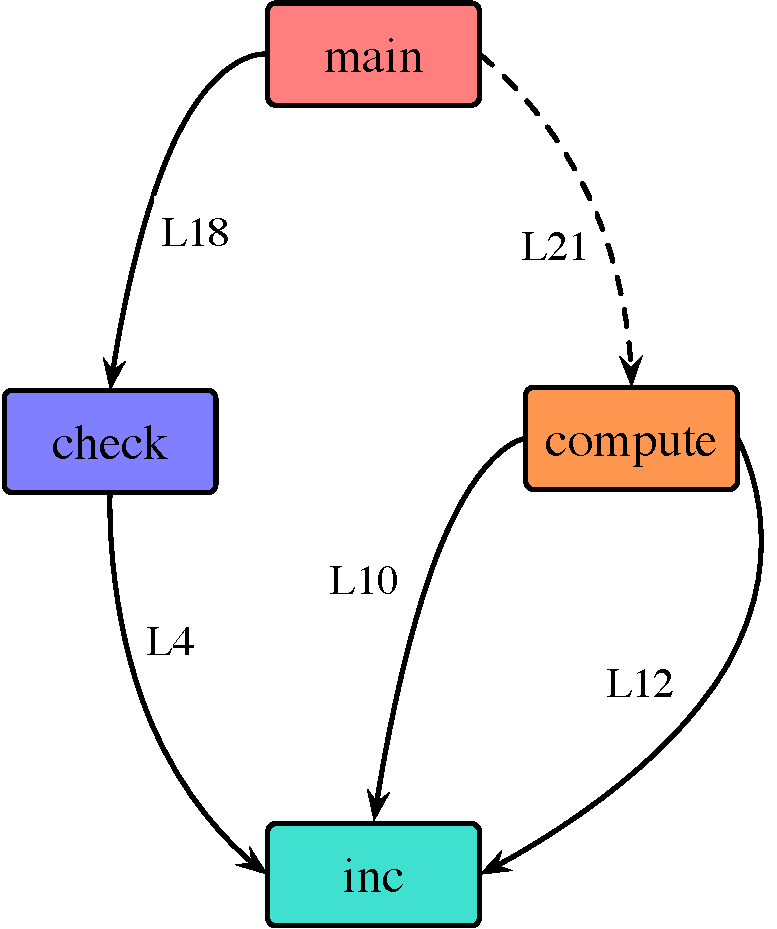
\includegraphics[width=.9\linewidth]{res/mtfuzz/callgraph.pdf}}
\caption{}\label{subfig:callgraph}
	\end{subfigure}\begin{subfigure}[b]{0.61\linewidth}
		\centering{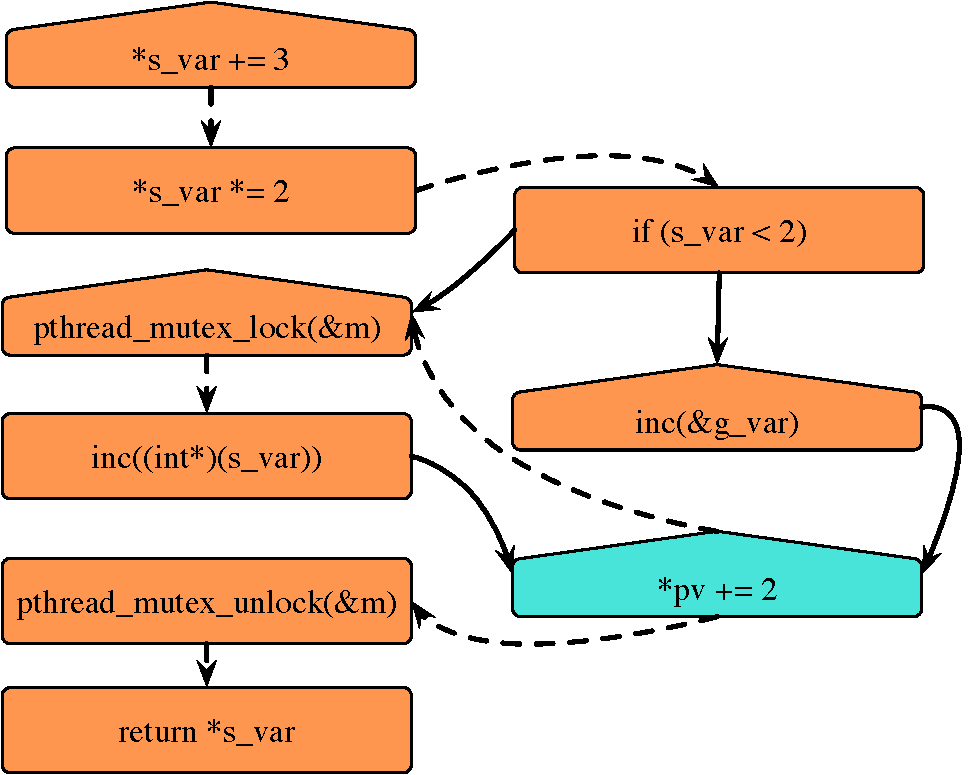
\includegraphics[width=.9\linewidth]{res/mtfuzz/transitions.pdf}}
\caption{}\label{subfig:transition}
	\end{subfigure}
	\caption{Thread-aware Callgraph (\ref{subfig:callgraph}) of Listing~\ref{lst:eg1} and its edge transitions in functions \texttt{compute} and \texttt{inc} (\ref{subfig:transition}).}
	\label{fig:eg_details}
\end{figure}





\begin{figure*}[ht]
    \centering
    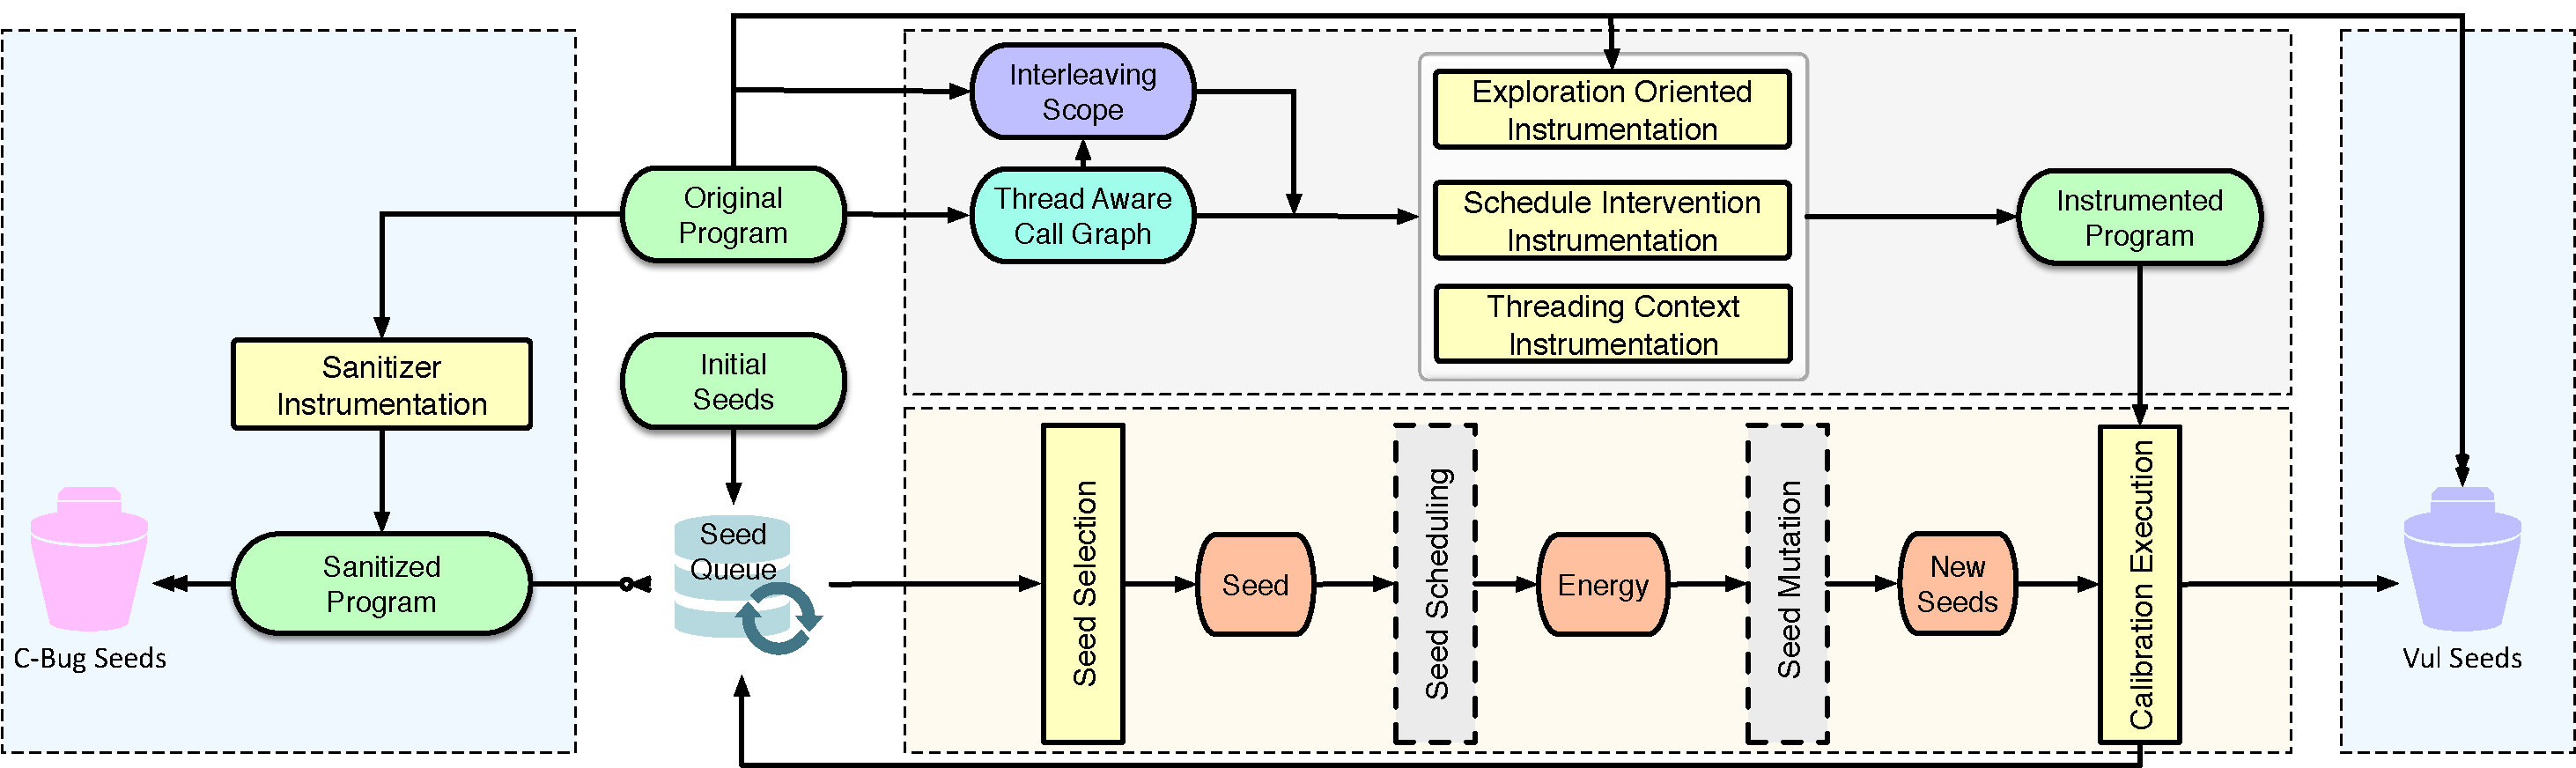
\includegraphics[width=0.93\textwidth]{res/mtfuzz/overview.pdf}
    \caption{Overall workflow of \mtfuzz.}
    \label{fig:workflow}
\end{figure*} 
\subsection{Low Diversity across Executions}\label{sec:afl_issue_mt}
When encountering a non-deterministic behavior seed, the only strategy of AFL is to execute the seeds more times. However, since the calibration execution is applied \emph{continuously} \Ncal times, the systematic level environment such as CPU usage, memory consumption, or other I/O status is prone to be similar~\cite{posixstd,tlpi}. This will decrease the entropy to diversify the actual scheduling. For example, in a calibration execution with $\Ncal=40$,  T1:\ding{172}$\rightarrow$T2:\ding{172}$\rightarrow$T1:\ding{173}$\rightarrow$T2:\ding{173} and T2:\ding{172}$\rightarrow$T1:\ding{172}$\rightarrow$T2:\ding{173}$\rightarrow$T1:\ding{173} may occur 15 and 20 times respectively, however interleavings such as T1:\ding{172}$\rightarrow$T1:\ding{173}$\rightarrow$T2:\ding{172}$\rightarrow$T2:\ding{173} only occurs 5 times, while there is no T2:\ding{172}$\rightarrow$T2:\ding{173}$\rightarrow$T1:\ding{172}$\rightarrow$T1:\ding{173} at all. In addition, since the running statistics are collected during calibration execution, this would also affect the decision in seed triaging. Ideally, we would like to keep as many distinct interleavings as possible since that marks the potential interleavings a seed can exhibit with different scheduling priorities.



\subsection{Our Solutions}
In order to improve the effectiveness of fuzzing multithreaded programs, we propose the following solutions.
\begin{enumerate}[{\bf S1}]
    \item Instead of equally choosing the the entry instruction of a basicblock as the deputy instruction, we apply a stratified exploration-oriented instrumentation by distinguish whether an instruction may happen-in-parallel with others~\cite{DBLP:conf/ppopp/DiS16,DBLP:conf/cgo/SuiDX16}.
This helps the fuzzer to track more thread-interleaving transitions.
    \item We instrument at the call site of thread-forking, locking, unlock, joining APIs and collect the thread and deputy instruction information to calculate the overall threading context per execution. This information is utilized to diversify the threading context of the seeds in the queue.
    \item We instrument at the entry of a thread start routine function a segment that can dynamically adjust the thread priority. It aims to increase the interleaving diversity during calibration execution.
\end{enumerate}






 \section{System Overview}

Fig.~\ref{fig:workflow} depicts the overall workflow of \mtfuzz. It contains three major components: (1) static-analysis-guided instrumentation (shown in the \emph{top center} area), (2) dynamic fuzzing (shown in the \emph{bottom center} area), and (3) concurrency bug replay (shown in the \emph{left and right} area). During instrumentation (~\S~\ref{sec:instrument}), we firstly compute the thread-aware ICFG (interprocedural control-flow graph) in \S~\ref{sec:tcg} for a multithreaded program (\ProgO). Based on this ICFG, we perform three categories of instrumentation: the one focusing on exploring more multithreading relevant paths (\S~\ref{sec:instrument_explore}), the one aiming to intervene the thread scheduling (\S~\ref{sec:instrument_schedule}) and the one that provides the threading context (\S~\ref{sec:instrument_thread_ctx}) to eventually produce the instrumented program~\Prog. During dynamic fuzzing~\S~\ref{sec:fuzz}, based on the instrumentation feedback, we apply seed selection (\S~\ref{sec:seed_select}), calibration execution (\S~\ref{sec:calibrate}) and seed triaging (\S~\ref{sec:seed_save}) that are turned for generating multithreading relevant seeds. Since the fuzzing procedure can only detect \emph{vulnerabilities} that are resulted from crashed seeds, we need a concurrency bug detector to replay with the generated seeds to see whether they can trigger certain concurrency violations; this will be covered in the evaluation section (\S~\ref{sec:eval_overall}).

\section{Static Instrumentation}\label{sec:instrument}
The static instrumentation is used to provide the thread-aware information for dynamic fuzzing.

As discussed in \S\ref{sec:afl_issue_mt}, the instrumentation strategy in existing GBFs is thread-unaware, which may miss transitions that caused by thread-interleaving for triggering vulnerabilities in multithreaded programs. Drawn from this insight, the precise fuzzing should distinguish program statements that may be access by concurrent threads, which requires ``finer-grained'' instrumentation to pay attention to the seeds that can capture the instruction transitions caused by interleaved threads, while deprioritize the seeds that exercise new paths only within a single thread.
We use results from static context-sensitive may-happen-in-parallel analysis~\cite{DBLP:conf/cgo/SuiDX16} to determine the thread-interleaving scope. The pointer analysis and lock analysis are enabled to further refine the scope to filter out the interleaving-free statements.
The static analysis is adopted as the preprocessing in~\S\ref{sec:preprocess} for our three categories of  instrumentation (\S~\ref{sec:instrument_explore}-\S~\ref{sec:instrument_thread_ctx}) for exploring new coverage, for intervening the schedule, and for guiding the seed selection procedure. 


\subsection{Preprocessing}\label{sec:preprocess}

\subsubsection{Thread-aware ICFG Generation}\label{sec:tcg}
We firstly apply Andersen's flow- and context-insensitive inclusion-based pointer analysis~\cite{Andersen94programanalysis} on the PUT. The points-to results are used to resolve indirect calls to eventually produce an interprocedural control-flow graph (ICFG). By taking into account the semantics of pthread APIs, we get an ICFG that is aware of the following multithreading information:
\begin{enumerate}[(1)]
    \item \TStart is the set of program sites that call thread-forking functions. This includes the explicit call to \func{pthread\_create}, or the \func{std::thread} constructor that internally uses \func{pthread\_create}, etc. These called functions, denoted as \FSStart, are extracted from the semantics of these forking sites.
\item \TEnd contains call sites for functions that mark the end of a multithreading execution. It includes the call sites of the pthread APIs such as \func{pthread\_join}, \func{pthread\_cancel}, \func{pthread\_exit}, etc.
    \item \TLock is the set of sites that call thread-locking functions such as \func{pthread\_mutex\_lock}, \func{pthread\_mutex\_trylock}, etc.
\item \TUnLock is the set of sites calling thread-unlocking functions such as \func{pthread\_mutex\_unlock} and \func{pthread\_rwlock\_unlock}.
    \item \TSharedVar is the set of variables that \emph{may be} shared among different threads. This includes the global variables and those variables that are passed from the threading fork sites \TStart.
\end{enumerate}

\subsubsection{Suspicious Interleaving Scope Extraction}\label{sec:extract}
Given a program that may run with multiple threads, we would prefer the instrumentation to collect various traces to reflect the interleavings. However, instrumentation always brings execution overhead to original programs, especially when adopting an intensive instrumentation strategy to cover all concerned sites.  Owing to the static information provided by the thread-aware ICFG in~\S\ref{sec:preprocess}, we know that multithreading interleavings may only happen on \emph{certain} program statements. We hereby use \mtiscope to denote the set of these statements and name it as \emph{suspicious interleaving scope}. Thus, the instrumentation is targeted on these statements. A statement $l$ is added into an thread-interleaving scope if there exists another statement $l'$, which may happen-in-parallel with $l$ and may access the same memory inferred by the pointer analysis, but not protected by the same lock.




In Listing~\ref{lst:eg1}, $\FSStart=\{\func{compute}\}$ based on the function call at Lines~\ref{line:main_thread_fork_1} and \ref{line:main_thread_fork_2}. We then get all the functions that may be (directly or indirectly) called by functions inside \FSStart, i.e., $\{inc, compute\}$ and the scope \mtiscope comes from Lines~\ref{line:g_var_def}, \ref{line:st_mt_func_start},
\ref{line:mt_func_start}$\sim$\ref{line:mt_func_end}.
We exclude the statements that do not access or modify the shared variables ${g\_var1}$, ${g\_var2}$, ${s\_var}$, 
which means we should exclude Lines~\ref{line:mt_func_lock} and \ref{line:mt_func_unlock}. In the end, the scope is determined as $\mtiscope=\{\ref{line:g_var_def},\ref{line:st_mt_func_start},
\ref{line:mt_func_start},\ref{line:mt_func_assign},\ref{line:mt_func_call},\ref{line:locked},\ref{line:mt_func_end}\}$. It is worth noting that line $\ref{line:locked}$ \emph{is} inside $\mtiscope$ since it may happen-in-parallel with lines~\ref{line:mt_func_start} and ~\ref{line:mt_func_assign}.


\subsection{Exploration-Oriented Instrumentation}\label{sec:instrument_explore}
With the knowledge of \mtiscope, we are able to instrument more stubs on these instructions inside the scope than the others, for exploring new ``transitions''. However, it is \emph{impractical} to instrument intensively on \emph{each instruction} inside \mtiscope since this still may greatly reduce the overall performance. It is also \emph{unnecessary} to do so --- although theoretically interleavings may happen everywhere at each instruction inside \mtiscope, in practice several instructions in one thread can still be executed subsequently. This means that we can skip some instructions for instrumentation, or instrument the instructions \emph{with a probability}.
We still need to instrument on the other parts of the program in case that the initial seeds do not cover the multithreading statements at all. Hence, we need the instrumentation to help explore more \emph{new} traces. Also similarly, we can \emph{skip} instrumentation on some instructions with certain probabilities.

\subsubsection{Instrumentation Probability Calculation}
We first calculate a \emph{base instrumentation probability} according to cyclomatic complexity. We use this since it has been demonstrated that bugs or vulnerabilities usually come from functions that have higher cyclomatic complexity~\cite{macabecc,vul_metric,fuzz_vul_metric}. For each function $\aFUNC$, we firstly calculate the complexity value: $M_c(\aFUNC) = E(\aFUNC) - N(\aFUNC) + 2$ where $E(\aFUNC)$ is the basicblock edge number of the function, $N(f)$ is the number of basicblocks. Intuitively, this value indicates the complexity of the function across its basicblocks. As 10 is considered to the preferred upper bound~\cite{macabecc}, we determine the base probability as
\begin{equation}
    \ccr{\aFUNC} = \min\big\{\frac{E(\aFUNC)-N(\aFUNC)+2}{10}, ~1.0\big\}
\end{equation}
We use $\stpn$ as the probability to \emph{selectively} instrument on the first instruction of a basicblock that is \emph{totally} outside the scope of multithreading environment, i.e., \emph{none of} the instructions inside this basicblock belongs to \mtiscope.
\begin{equation}
    \stp{\aFUNC} = \max\big\{\ccr{\aFUNC}, ~\stpnO\big\}
\end{equation}
where $0<\stpnO<1$. Empirically, we set $\stpnO=0.5$.

On the other hand, for each basicblock \aBB inside the given function~\aFUNC, we calculate the total number of instructions $N(\aBB)$, and the total number of memory operation instructions  $N_m(\aBB)$, e.g., load/store operations, or built-in memory function calls such as \func{memcpy}, \func{strncat}, \func{malloc}, \func{free}, etc. 
Then for each of the instructions, we instrument based on the probability as:
\begin{equation}
    \mtp{\aFUNC}{\aBB} = \max\big\{\ccr{\aFUNC}\cdot\frac{N_m(\aBB)}{N(\aBB)}, ~\mtpnO \big\}\end{equation}
where $\mtpnO$ is a factor satisfying $0<\mtpnO<1$ and defaults to $0.33$.

\subsubsection{Instrumentation Algorithm}
The exploration-oriented instrumentation algorithm is described in Algo.~\ref{algo:inst_explore}. It iterates each function inside a program. For each basicblock \aBB in function \aFUNC, we firstly get the intersection of the instructions inside \aBB and \mtiscope. If this intersection \mtiscope(\aBB) is empty, it instruments the \emph{first instruction} of \aBB with a probability of \emph{\stpn(\aFUNC)}. Otherwise, for the first instruction in \aBB, we always instrument it (instrument with probability of 1.0); for the other instructions, if they are inside \mtiscope, we instrument them with a probability of \mtp{\aFUNC}{\aBB}. We will refer our selection of deputy instructions as \MTIns.

\begin{algorithm}[t]
  \SetKwInOut{Input}{input}
  \SetKwInOut{Output}{output}
\Input{Target program \var{P}, suspicious interleaving scope~\mtiscope}\Output{Program \var{P} instrumented with exploration stubs}
\For{\var{\aFUNC} $\in$ \var{P}}{
  \For{\var{\aBB} $\in$ \aFUNC}{
    $\mtiscope(\aBB) = \mtiscope\cap~\aBB$\;
    \uIf{$\mtiscope(\aBB)~!\!=\emptyset$}{
      \For{\aINSTR $\in$ \aBB}{
        \uIf{\func{is\_first\_instr(\aINSTR, \aBB)}}{
          exploration\_instrument(\aINSTR, 1.0)\;
        }
        \ElseIf{$\aINSTR\in\mtiscope$}{
          exploration\_instrument\big(\aINSTR, \mtp{\aFUNC}{\aBB}\big)\;
        }
      }      
    }\Else{
      \For{\aBB $\in$ \aFUNC}{
        \aINSTR = get\_first\_inst(\aBB)\;
        exploration\_instrument\big(\aINSTR, \stp{\aFUNC}\big)\;
      }
    }
  }
}
\caption{Exploration-Oriented Instrumentation}\label{algo:inst_explore}
\end{algorithm}

\subsubsection{Properties of the Coverage in \MTIns}

First, for both \AFLIns and \MTIns, the coverage is shaped by the transitions between deputy instructions. The difference is that we use a stratified instrumentation strategy to focus on the interleavings introduced by multithreading scheduling. Compared to \AFLIns, \MTIns instruments less on the single threading program statements, while applies more instrumentation to explore more interleavings across different threads with certain probabilities.

Second, mistakenly instrumenting on non-entry instructions that are not in \mtiscope will \emph{only introduce runtime overhead}, but \emph{never} help to keep more seeds.
This can be proved by the fact that GBFs keep new seeds based on ``new transitions'', however the ``new transitions'' conditions are always the regardless of whether the exercised instruction are instrumented. 
In this sense, we may expect that there will not be seeds \emph{accidentally} added into the seed queue due to over-estimation of \mtiscope. 

Thirdly, \MTIns's strategy to tracking multithreading interleaving \emph{is} useful and it is worth instrumenting more on these instructions that may be executed parallelly with other instructions. The major reason is that we can expect to have more valuable seeds. Same as other GBFs, we still rely on observations of ``new transitions'' to keep seeds, and \MTIns tends to keep more seeds that execute thread-interleaving, regardless of the precision of the calculated \mtiscope. First, it means that more seeds in the seed queue for fuzzing have executed the multithreading code segments, instead of having failed the validation check quite earlier. Hence, these seeds can execute the ``deeper part'' of a multithreaded program. When they are mutated, compared with those seeds that fail the validity check, there is a higher chance that the newly generated seeds from these seeds also pass the check and exercise different part of the multithreading segments. Therefore, the high ratio of seeds that can execute multithreading segments already indicates the seeds are probably of high qualities. Second, since seeds usually exhibit some preference in executing with certain interleavings, some thread-interleavings are more ``stable'', they may be just like the regular transitions inside single thread.

Finally, since \MTIns only selectively instruments the instructions inside \mtiscope with a probability of at most \mtpnO, we avoid over-emphasizing thread-interleaving induced transitions, as well as seek a balance between runtime instrumentation overhead and coverage feedback. 













\subsection{Schedule Intervention Instrumentation}\label{sec:instrument_schedule}

Without specifying any schedule policy or priority, the operation systems usually determine the actual schedule dynamically~\cite{tlpi,posixstd}. As mentioned in \S\ref{sec:afl_issue_mt}, without scheduling intervention the calibration execution during fuzzing may not exhibit diverse interleavings, which is unsatisfactory for covering new transitions. 

POSIX compliant systems such as Linux
usually provide the APIs to control the low level process or thread schedulings~\cite{posixstd,tlpi}.
In order to intervene the interleavings during the execution of the multithreading program, we adjust the thread priorities.
This heavily resorts to the POSIX API \func{pthread\_setschedparam}. Our intervention of scheduling follows two principles: 1) the intervened schedule should be possible to happen in reality without this intervention; 2) the schedule should make the interleavings more diverse. We therefore instrument a function call \rtifunc at the start of the thread routine. This instrumented function does two things:
\begin{enumerate}[(1)]
    \item For each newly mutated test input, it calls \func{pthread\_self} in the entry of \FSStart to collect the runtime thread IDs. This serves two purposes.
    First, it marks the entering of the multithreading region in order to inform the fuzzer that the execution trace has covered the thread spawning statements.
    Second, each collected thread ID will also be associated with a unique number \ntid starting from $1,2,\ldots$, which will be used to calculate the threading context in \S\ref{sec:instrument_thread_ctx}.
    \item During the calibration execution~\S~\ref{sec:calibrate}, whenever the thread comes to call \rtifunc, it changes the schedule policy to \emph{SCHED\_RR}, and assigns a \emph{ranged random value} to its priority.
    We make the priority value to be \emph{uniformly distributed random} in order to diversify the combinations among threads.
\end{enumerate}

\subsection{Threading Context Instrumentation}\label{sec:instrument_thread_ctx}
We also apply an instrumentation to track the threading context, which is used to collect thread relevant context for additional feedback during seed selection.
This context is collected at the call site of $\FSThread=\{\TLock, \TUnLock, \TEnd\}$, each of which has the form $\threadCtxn=\threadCtx{\iloc}{\ntid}$. Here \iloc is the labeling value of previous deputy instruction (c.f. \S\ref{sec:afl_issue_ins} and \S~\ref{sec:instrument_explore}). \ntid is obtained by getting the value of the key identified by current thread ID from the thread ID map collected at \S\ref{sec:instrument_schedule}. For each function in \FSThread, we keep a sequence of context $\langle\threadCtxn{_1}(f),\ldots,\threadCtxn{_n}(f)\rangle$,$f\in\FSThread$; and at the end of each execution we calculate a hash value $H(f)$ for each of them. The tuple $\tctxSign=\big\langle H(\TLock),H(\TUnLock),H(\TEnd)\big\rangle$ is a \emph{context signature} that determines the overall threading context of a specific execution. Essentially, this is a sampling on these thread relevant APIs to track the overall thread information and transitions of a particular run. As we shall see later, this plays an important role in seed selection (\S\ref{sec:seed_select}).

Till now, we have done all the static instrumentation. Note that we manage to keep the original programs' semantics, and hence the execution behaviors are basically the same as the original one.

\section{Dynamic Fuzzing}\label{sec:fuzz}
The dynamic fuzzing loop follows a typical GBF procedure as described in Algo.\ref{algo:gbf}. We improve the procedures of seed selection (\S\ref{sec:seed_select}),
calibration execution (\S\ref{sec:calibrate}) and seed triaging (\S\ref{sec:seed_save}) to fit specially for fuzzing multithreaded programs, based on the instrumentation information provided in \S\ref{sec:instrument}.

\subsection{Seed Selection}\label{sec:seed_select}

Seed selection decides which seeds to be mutated next. In practice, this problem is reduced to whether the next seed $t$ at the queue header will be selected into $\Seeds$, which is depicted by Algo.~\ref{algo:select_seed}.






During seed selection, in addition to following AFL's strategy by using \func{has\_new\_trace(\Seeds)} to  checking whether \Seeds contains a ``favored seed'' $t$ that covers a new transition (\func{cov\_new\_trace(t)}=true), we also check whether there is at least one seed in \Seeds that reaches the multithreading code (i.e., \func{has\_new\_mt\_ctx(\Seeds)}). If either of the conditions is satisfied, it means there are some ``interesting'' seeds.
Specifically, if the seed has a new threading context, the algorithm directly returns  true. If it covers a new trace, it has a probability of \probYNT to be selected; otherwise, the probability is \probYNN. Last, if no interesting seeds in \Seeds are interesting at all, the algorithm selects with a probability of \probNNN. Analogous to AFL's selection strategy, we set $\probYNT=0.95$, $\probYNN=0.01$, $\probNNN=0.15$.

To implement $\func{cov\_new\_mt\_ctx(t)}$, we track the context of calling a multithreading API in $\FSThread=\{\TEnd, \TLock, \TUnLock\}$ (c.f. \S\ref{sec:instrument_thread_ctx}) and check whether the  context signature \tctxSign has been met before ---  when \tctxSign is new, $\func{cov\_new\_mt\_ctx(t)}=true$; otherwise, $\func{cov\_new\_mt\_ctx(t)}=false$. Note that $\func{cov\_new\_trace(t)=true}$ does not imply $\func{cov\_new\_mt\_ctx(t)=true}$. The reason is that (1) we cannot instrument inside the body of thread API functions in \FSThread, and hence $\func{cov\_new\_trace}$ cannot track the transitions; (2) $\func{cov\_new\_mt\_ctx}$ also depends on the thread IDs that $\func{cov\_new\_trace}$ is unaware of.  












\begin{algorithm}[t]
\SetKwInOut{Input}{input}
  \SetKwInOut{Output}{output}
  \Input{Seed queue~\Seeds, current seed in queue $t$}
  \Output{whether $t$ will be selected in this round}
  \uIf{has\_new\_mt\_ctx(\Seeds) \text{||} has\_new\_trace(\Seeds)}{
      \uIf{cov\_new\_mt\_ctx($t$)}{
        \Return{true}\;
      } \uElseIf{\func{cov\_new\_trace($t$)}}{
        \Return{\func{select\_with\_prob(\probYNT)}}\;
      } \Else{
        \Return{\func{select\_with\_prob(\probYNN)}}\;
      }
  }\Else{
    \Return{\func{select\_with\_prob(\probNNN)}}\;
  }
  \caption{Algorithm to Select Next Seed}\label{algo:select_seed}
\end{algorithm}







\subsection{Calibration Execution}\label{sec:calibrate}
Multithreaded programs introduce non-deterministic behaviors when different interleavings are involved.
As seen in Algo.~\ref{algo:gbf}, for a mutated seed, a GBF typically executes the PUT with multiple times. 
Owing to~\rtifunc, we are now able to tell whether the current non-deterministic behavior is relevant with a multithreading execution. In fact, since we focus on multithreading only, based on the times of the threading forking operations the fuzzer has observed, the fuzzer can distinguish the calibration on those seeds that have non-deterministic behaviors purely by checking whether the execution traces have touched the threading relevant regions. Further, if we know that a seed may have more distinct values of \tctxSign (the number of distinct values for seed $t$ is denoted as \Nmt(t)), there will be more interleavings. To determine the calibration times~\Ncal, we rely on \Nmt. In AFL, the calibration times is calculated by the equation below:
\begin{equation}
    \Ncal(t) = \NcalO + \NcalV\cdot\NcalB \label{eq:afl_cal}
\end{equation}
where \NcalO is the initial calibration times, \NcalV is a constant as the ``bonus'' calibration times for non-deterministic runs, and $\NcalB\in\{0,1\}$. \NcalB=0 if none of the \NcalO calibration runs show non-deterministic behaviors, otherwise \NcalB=1. We argue this to specially fit for multithreading setting. 
\begin{equation}
    \Ncal(t) = \NcalO + \texttt{min}\big\{\NcalV, \NcalO\cdot\Nmt(t)\big\}
\end{equation}
In both AFL and \mtfuzz, $\NcalO=8$, $\NcalV=32$.
For all the \Ncal calibration runs, we track their execution traces and count how many different traces (\NcalTrace) it exhibits. 


\subsection{Seed Triaging}\label{sec:seed_save}
This handles how to categorize the seeds after calibration execution. \mtfuzz still follows the workflow at Lines~\ref{line:algo:triage_start}$\sim$\ref{line:algo:triage_end} in Algo.~\ref{algo:gbf}: if there is a crash, we mark these seeds as vulnerable; if the seed covers new transitions, we append it to the queue. One major difference is that these ``seemingly normal'' seeds may actually have concurrent bugs. These will be handled in the replaying procedure (\S~\ref{sec:eval_overall}) after fuzzing. To provide a hint on how many times to be executed on a specific seed during replaying, we keep \NcalTrace statistics.



\begin{table*}[ht]
\caption{Static information of the 12 evaluated programs.}
\label{tbl:bm_stats}
\tiny
\begin{tabular}{c"c|c|c|c"c|c|c|c|r}
\thickhline
\textbf{ID} &\textbf{Project} & \textbf{MT Type} & \textbf{Command Line Options}  & \textbf{\begin{tabular}[c]{@{}c@{}}Binary\\ Size\end{tabular}} &  \textbf{$T_{pp}$} & \textbf{$N_{B}$} & \textbf{$N_{I}$} & \textbf{$N_{ii}$} & \textsf{$\frac{N_{ii}-N_{B}}{N_{B}}$} \\ \thickhline
\textbf{lbzip2-c} & lbzip2-2.5 & native & \pbin{lbzip2} -k -t -9 -z -f -n4 FILE & 377k & 7.1s & 4010 & 24085 & 6208 & 54.8\% \\  \hline
\textbf{pbzip2-c} & pbzip2-v1.1.13 & native & \pbin{pbzip2} -f -k -p4 -S16 -z FILE & 312k & 0.9s & 2030 & 8345 & 2151 & 6.0\% \\  \hline
\textbf{pbzip2-d} & pbzip2-v1.1.13 & native & \pbin{pbzip2} -f -k -p4 -S16 -d FILE & 312k & 0.9s & 2030 & 8345 & 2151 & 6.0\% \\ \hline
\textbf{pigz-c} & pigz-2.4 & native & \pbin{pigz} -p 4 -c -b 32 FILE & 117k & 5.0s & 3614  & 21022 & 5418 & 49.9\% \\ \hline
\textbf{pxz-c} & pxz-4.999.9beta & OpenMP & \pbin{pxz} -c -k -T 4 -q -f -9 FILE & 42k & 1.2s & 3907 & 30205 & 7877 & 101.6\% \\ \hline
\textbf{xz-c} & XZ-5.3.1alpha & native & \pbin{xz} -9 -k -T 4 -f FILE & 182k & 8.4s & 4892 & 34716 & 8948 & 82.9\% \\ \hline
\textbf{gm-cnvt} &  GraphicsMagick-1.4 & OpenMP & \pbin{gm} convert -limit threads 4  FILE out.bmp & 7.6M & 224.4s & 63539 & 383582 & 98580 & 55.1\% \\ \hline
\textbf{im-cnvt} & ImageMagick-7.0.8-7 & OpenMP & \pbin{convert} -limit thread 4 FILE out.bmp & 19.4M & 434.2s & 128359 & 778631 & 200108 & 55.9\% \\ \hline
\textbf{cwebp} & libwebp-1.0.2 & native & \pbin{cwebp} -mt FILE -o out.webp & 1.8M & 56.3s & 12117 & 134824 & 33112 & 173.3\%\\ \hline
\textbf{vpxdec} & libvpx-v1.3.0-5589 & native & \pbin{vpxdec} -t 4 -o out.y4m FILE & 3.8M & 431.6s & 31638 & 368879 & 93400 & 195.2\% \\ \hline
    \textbf{x264} & x264-0.157.2966 & native & \pbin{x264} --threads=4 -o out.264 FILE & 6.4M & 1701.0s & 38912 & 410453 & 103926 & 167.1\% \\ \hline
\textbf{x265} & x265-3.0\_Au+3 & native & \pbin{x265} --input FILE --pools 4 -F 2 -o & 9.7M & 78.3s & 22992 & 412555 & 89408 & 288.9\% \\ \thickhline
\end{tabular}
\end{table*}



%\begin{table*}[ht]
%\caption{Overall fuzzing and replaying results on \mtfuzz, \mtfuzzc and AFL.}
%\label{tbl:eval_overall}
%\centering
%\tiny
%\begin{tabular}{|c|c|c|c|c|c|c|c|c|c|c|c|c|c|c|c|c|c|c|c|c|c|}
%\hline
%\multirow{3}{*}{\textbf{ID}} & \multicolumn{7}{c|}{\textbf{\mtfuzz}} & \multicolumn{7}{c|}{\textbf{\mtfuzzc}} & \multicolumn{7}{c|}{\textbf{AFL}} \\ \cline{2-22}
%& \multicolumn{3}{c|}{\textbf{Gen Tests}} & \multicolumn{3}{c|}{\textbf{Vuls}} & \multirow{2}{*}{\textbf{\begin{tabular}[c]{@{}c@{}}C-\\ Bug\end{tabular}}} & \multicolumn{3}{c|}{\textbf{Gen Tests}} & \multicolumn{3}{c|}{\textbf{Vuls}} & \multirow{2}{*}{\textbf{\begin{tabular}[c]{@{}c@{}}C-\\ Bug\end{tabular}}} & \multicolumn{3}{c|}{\textbf{Gen Tests}} & \multicolumn{3}{c|}{\textbf{Vuls}} & \multirow{2}{*}{\textbf{\begin{tabular}[c]{@{}c@{}}C-\\ Bug\end{tabular}}}  \\ \cline{2-7} \cline{9-14} \cline{16-21}
%& \textbf{\testsALL} & \textbf{\testsMT} & \textbf{\textbf{\testsRatio}}  & \textbf{\vulsNUM} &  \textbf{\vulsMT} & \textbf{\vulsST} &  & \textbf{\testsALL} & \textbf{\testsMT} & \textbf{\testsRatio} & \textbf{\vulsNUM} & \textbf{\vulsMT}  & \textbf{\vulsST} &  & \textbf{\testsALL} & \textbf{\testsMT} & \textbf{\testsRatio} & \textbf{\vulsNUM} & \textbf{\vulsMT} & \textbf{\vulsST} &  \\ 
%\hline
%\textbf{lbzip2-c} & \gres{4503 } & \gres{1637} & \gres{36.4\%} &  0    &   0   &   0 & 1                 &  4155   &  1352  &  32.5\%  & 0   & 0 & 0 & 1                 &  3350   & 753   &  22.5\%  &  0   & 0 & 0 & 1          \\ \hline
%\textbf{pbzip2-c} & \gres{253  } & \gres{78  } & \gres{30.8\%} &  4    &   \gres{1}   &  0 & 0           &  227    &  59    &  26.0\%  & \gres{6}   & \gres{1} & 0 & 0   &  175    & 50    &  28.6\%  &  0   & 0 & 0 & 0          \\ \hline
%\textbf{pbzip2-d} & \gres{1231 } & \gres{47  } & \gres{3.8\% } &  \gres{5}    &   \gres{1} & 0  & 0      &  982    &  11    &  1.2\%   & 0   & 0 & 0 & 0                 &  926    & 7     &  0.8\%   &  0   & 0 & 0 & 0          \\ \hline
%\textbf{pigz-c}   & \gres{921  } & \gres{789 } & \gres{85.7\%} &  0    &   0   &   0 & 1                 &  836    &  673   &  80.5\%  & 0   & 0 & 0 & 1                 &  737    & 592   &  80.3\%  &  0   & 0 & 0 & 1          \\ \hline
%\textbf{pxz-c}    & \gres{3658 } & \gres{2523} & \gres{69.0\%} &  0    &   0   &   0 & 0                 &  2804   &  1675  &  59.7\%  & 0   & 0 & 0 & 0                 &  2305   & 958   &  41.6\%  &  0   & 0 & 0 & 0          \\ \hline
%\textbf{xz-c}     & \gres{1598 } & \gres{493 } & \gres{30.9\%} &  0    &   0   &   0 & 0                 &  1359   &  268   &  19.7\%  & 0   & 0 & 0 & 0                 &  1327   & 257   &  19.4\%  &  0   & 0 & 0 & 0          \\ \hline
%\textbf{gm-cnvt}  & \gres{4677 } & \gres{3265} & \gres{69.8\%} &  0    &   0   &   0 & \gres{5}          &  4036   &  2092  &  51.8\%  & 0   & 0 & 0 & 4                 &  3921   & 1872  &  47.7\%  &  0   & 0 & 0 & 3          \\ \hline
%\textbf{im-cnvt}  & \gres{4355 } & \gres{3671} & \gres{84.3\%} &  \gres{21} &  \gres{4} &  1 & \gres{3}  &  4028   &  3257  &  80.9\%  & 14  & 2 & 1 & 3                 &  3289   & 2460  &  74.8\%  &  8   & 2 & 1 & 2          \\ \hline
%\textbf{cwebp}    & \gres{5701 } & \gres{3347} & \gres{58.7\%} &  8    &   0   &   1 & 0                 &  5549   &  3095  &  55.8\%  & \gres{11}  & 0 & 1 & 0          &  4755   & 2234  &  47.0\%  &  9   & 0 & 1 & 0          \\ \hline
%\textbf{vpxdec}   & \gres{14665} & \gres{3656} & \gres{24.9\%} &  336  &   \gres{2}   &   2 & \gres{3}   &  13927  &  3302  &  23.7\%  & \gres{364} & 1 & 2 & 1          &  13046  & 3117  &  23.9\%  &  345 & 1 & 2 & 1          \\ \hline
%\textbf{x264}     & \gres{5023 } & \gres{4832} & \gres{96.2\%} &  \gres{7}    &   1   &   0 & \gres{9}   &  4457   &  4197  &  94.2\%  & 6   & 1 & 0 & 6                 &  4465   & 4252  &  95.2\%  &  3   & 1 & 0 & 4          \\ \hline
%\textbf{x265}     & 6433  & \gres{5012}  & \gres{78.0\%}  &  29   &   0   &   1 & 0                           &  \gres{6743} & {5007}  &  74.3\%  & 43  & 0 & 1 & 0      &  6420   & 4701  &  73.2\%  &  \gres{49}  & 0 & 1 & 0   \\ \hline
%\end{tabular}
%\end{table*}



\begin{table}[h]
\caption{Fuzzing and Replaying Results on \AFL}
\label{tbl:afl_results}
\centering
\footnotesize
\begin{tabular}{|c|c|c|c|c|c|c|c|c|}
\thickhline
\multicolumn{2}{|c|}{\multirow{2}{*}{\textbf{ID}}} & \multicolumn{3}{c|}{\textbf{Gen Tests}} & \multicolumn{3}{c|}{\textbf{Vuls}} & \multirow{2}{*}{\textbf{C-Bugs}} \\ \cline{3-8}
\multicolumn{2}{|c|}{} & \textbf{\testsALL} & \textbf{\testsMT} & \textbf{\textbf{\testsRatio}}  & \textbf{\vulsNUM} &  \textbf{\vulsMT} & \textbf{\vulsST} &  \\ \hline
\multirow{12}{*}{\textbf{\mtfuzz}}     & \textbf{lbzip2-c} &  3350   & 753   &  22.5\%  &  0   & 0 & 0 & 1   \\ \cline{2-9} 
    & \textbf{pbzip2-c} &  175    & 50    &  28.6\%  &  0   & 0 & 0 & 0    \\ \cline{2-9} 
    & \textbf{pbzip2-d} &  926    & 7     &  0.8\%   &  0   & 0 & 0 & 0  \\ \cline{2-9} 
    & \textbf{pigz-c} &  737    & 592   &  80.3\%  &  0   & 0 & 0 & 1   \\ \cline{2-9} 
    & \textbf{pxz-c} &   2305   & 958   &  41.6\%  &  0   & 0 & 0 & 0  \\ \cline{2-9} 
    & \textbf{xz-c} &  1327   & 257   &  19.4\%  &  0   & 0 & 0 & 0  \\ \cline{2-9} 
    & \textbf{gm-cnvt} &  3921   & 1872  &  47.7\%  &  0   & 0 & 0 & 3 \\ \cline{2-9} 
    & \textbf{im-cnvt} &  3289   & 2460  &  74.8\%  &  8   & 2 & 1 & 2  \\ \cline{2-9} 
    & \textbf{cwebp} &  4755   & 2234  &  47.0\%  &  9   & 0 & 1 & 0  \\ \cline{2-9} 
    & \textbf{vpxdec} &  13046  & 3117  &  23.9\%  &  345 & 1 & 2 & 1  \\ \cline{2-9} 
    & \textbf{x264} &  4465   & 4252  &  95.2\%  &  3   & 1 & 0 & 4  \\ \cline{2-9} 
    & \textbf{x265} &  6420   & 4701  &  73.2\%  &  \gres{49}  & 0 & 1 & 0  \\ \thickhline
\multirow{12}{*}{\textbf{\mtfuzz}}    & \textbf{lbzip2-c} &  4155   &  1352  &  32.5\%  & 0   & 0 & 0 & 1  \\ \hline
    & \textbf{pbzip2-c} &  227    &  59    &  26.0\%  & \gres{6}   & \gres{1} & 0 & 0   \\ \hline
    & \textbf{pbzip2-d} &  982    &  11    &  1.2\%   & 0   & 0 & 0 & 0   \\ \hline
    & \textbf{pigz-c} & \gres{921  } & \gres{789 } & \gres{85.7\%} &  0    &   0   &   0 & 1  \\ \hline
    & \textbf{pxz-c} &  2804   &  1675  &  59.7\%  & 0   & 0 & 0 & 0  \\ \hline
    & \textbf{xz-c} &  1359   &  268   &  19.7\%  & 0   & 0 & 0 & 0  \\ \hline
    & \textbf{gm-cnvt} & \gres{4677 } & \gres{3265} & \gres{69.8\%} &  0    &   0   &   0 & \gres{5} \\ \hline
    & \textbf{im-cnvt} &  4036   &  2092  &  51.8\%  & 0   & 0 & 0 & 4  \\ \hline
    & \textbf{cwebp} &  5549   &  3095  &  55.8\%  & \gres{11}  & 0 & 1 & 0  \\ \hline
    & \textbf{vpxdec} &  13927  &  3302  &  23.7\%  & \gres{364} & 1 & 2 & 1  \\ \hline
    & \textbf{x264} &  4457   &  4197  &  94.2\%  & 6   & 1 & 0 & 6  \\ \hline
    & \textbf{x265} &  \gres{6743} & {5007}  &  74.3\%  & 43  & 0 & 1 & 0  \\ \thickhline
\multirow{12}{*}{\textbf{\mtfuzz}}    & \textbf{lbzip2-c} & \gres{4503 } & \gres{1637} & \gres{36.4\%} &  0    &   0   &   0 & 1   \\ \hline
    & \textbf{pbzip2-c} & \gres{253  } & \gres{78  } & \gres{30.8\%} &  4    &   \gres{1}   &  0 & 0   \\ \hline
    & \textbf{pbzip2-d} & \gres{1231 } & \gres{47  } & \gres{3.8\% } &  \gres{5}    &   \gres{1} & 0  & 0  \\ \hline
    & \textbf{pigz-c} & \gres{921  } & \gres{789 } & \gres{85.7\%} &  0    &   0   &   0 & 1  \\ \hline
    & \textbf{pxz-c} & \gres{3658 } & \gres{2523} & \gres{69.0\%} &  0    &   0   &   0 & 0  \\ \hline
    & \textbf{xz-c} & \gres{1598 } & \gres{493 } & \gres{30.9\%} &  0    &   0   &   0 & 0  \\ \hline
    & \textbf{gm-cnvt} & \gres{4677 } & \gres{3265} & \gres{69.8\%} &  0    &   0   &   0 & \gres{5} \\ \hline
    & \textbf{im-cnvt} & \gres{4355 } & \gres{3671} & \gres{84.3\%} &  \gres{21} &  \gres{4} &  1 & \gres{3}  \\ \hline
    & \textbf{cwebp} & \gres{5701 } & \gres{3347} & \gres{58.7\%} &  8    &   0   &   1 & 0  \\ \hline
    & \textbf{vpxdec} & \gres{14665} & \gres{3656} & \gres{24.9\%} &  336  &   \gres{2}   &   2 & \gres{3}  \\ \hline
    & \textbf{x264} & \gres{5023 } & \gres{4832} & \gres{96.2\%} &  \gres{7}    &   1   &   0 & \gres{9}  \\ \hline
    & \textbf{x265} & 6433  & \gres{5012}  & \gres{78.0\%}  &  29   &   0   &   1 & 0  \\ \hline
    & \end{tabular}
\end{table}

 
\section{Evaluation}

We develop \mtfuzz upon \FOT and SVF~\cite{Sui:2016:SVF,DBLP:conf/ppopp/DiS16,DBLP:conf/cgo/SuiDX16}. 
The static instrumentation component utilizes the LLVM analysis while the 
thread-aware callgraph construction leverages SVF's inter-procedural value-flow 
analysis. In total this static part has around 3000 lines of C/C++ code. Also, 
we modify \FOT's fuzzing engine with about 800 lines of C code. And the replay part 
takes additional 1500 lines of Python code. We archive all the supporting materials 
at~\cite{mtfuzz-webpage}. These include the initial 
fuzzing seeds, the source code, and the findings of our evaluation.

Specifically, we design the following research questions to conduct our evaluation:
\begin{enumerate}[{\bf RQ1}]
    \item Can \mtfuzz generate seeds that can trigger more non-deterministic 
			program behaviors?
    \item What is the capability of \mtfuzz in detecting vulnerabilities?
    \item Can the generated seeds help third-party bug detector to find more 
			concurrency faults?
\end{enumerate}

\subsection{Evaluation Setup}
Our experiments are conducted on an Intel(R) Xeon(R) Platinum
8151 CPU @ 3.40GHz with 28 cores, running a 64-bit Ubuntu 18.04
LTS system; during experiments, we use 24 cores and retain 4 cores
for other processes.

\subsubsection{Settings of the fuzzers}
We set up three fuzzers for evaluation:
\begin{enumerate}[1)]
\item \textbf{AFL} is the current state-of-the-art GBF with \AFLIns instrumentation 
and the thread-unaware fuzzing strategies. To the best of our knowledge, there are no 
other open-source fuzzers that targets multithreaded programs. Meanwhile, evolved AFL 
shows comparable performance with recent techniques~\cite{ccs18_eval_fuzzing,Shastry:LNCS2017:Orthrus}. 
Therefore, we use AFL as the baseline fuzzer.

\item \textbf{\mtfuzzc} enhances AFL with the schedule intervention instrumentation 
(\S\ref{sec:instrument_schedule}) and threading context instrumentation\S\ref{sec:instrument_thread_ctx}) and all the dynamic strategies (\S\ref{sec:fuzz}) .

\item \textbf{\mtfuzz} is our proposed fuzzer. It has all the static and dynamic 
strategies proposed in \S\ref{sec:instrument} and \S\ref{sec:fuzz}. \mtfuzz differs
from \mtfuzzc only on the exploration-oriented instrumentation --- the latter uses AFL's instrumentation strategy \AFLIns.
\end{enumerate}

During evaluation, all the fuzzers are executed in the ``fidgety'' mode as
suggested in~\cite{FidgetyAFL}. We also disable AFL's CPU affinity binding
strategy. This is because that the threads in multithreading pro-
grams are intended to be mapped in different cores and execute in
parallel in order to boost overall performance; setting the CPU affinity will make all these threads bound to one CPU core. In practice, setting CPU affinity frequently makes fuzzing procedure fail due to heavy loads.



\subsubsection{Statistics of the evaluation dataset}

The dataset for evaluation consists of the following real-world software projects.
\begin{enumerate}[1)]
    \item Parallel compress/decompress utilities including \textbf{pigz}, \textbf{lbzip2}, 
			\textbf{pbzip2}, \textbf{xz} and \textbf{pxz}. These tools have been present in 
			GNU/Linux distributions for many years and are integrated
into the widely used GNU \textsf{tar} utility.
    \item \textbf{ImageMagick} and \textbf{GraphicsMagick} are two widely used soft-
ware suites to display, convert, edit images files.
    \item \textbf{libvpx} and \textbf{libwebp} are two WebM projects. They are used by
mainstream browsers like Google Chrome, Firefox, and Opera.
    \item \textbf{x264} and \textbf{x265} are two most established video encoders for
H.264/AVC and HEVC/H.265 formats respectively.
\end{enumerate}

All these software systems have been intensively tested by AFL, LibFuzzer, or added into Google's OSS-Fuzz project. We try to use their \emph{latest} versions at the 
time of evaluation; the only exception is libvpx, which we use version v1.3.0-5589 to 
reproduce vulnerabilities and concurrency bugs.


Table~\ref{tbl:bm_stats} lists the statistical data of the benchmarks. The first two 
columns show the benchmark names and their host software projects. The third column
represents the multithreading implementation --- either the OpenMP~\cite{openmp} 
APIs or the standard pthread library. The next column specifies the command line options.


The rest columns state the static instrumentation data. The ``Binary Size'' column 
calculates the sizes of the instrumented binaries. Column $T_{pp}$ records the 
preprocessing time (c.f.~\S\ref{sec:preprocess}). The program \emph{vpxdec} cost the 
most time --- about 30 minutes. The last three columns $N_B$, $N_I$, and $N_{ii}$ 
depict the number of basic blocks, the number of total instructions, and the number 
of included instructions for \mtfuzz instrumentation (c.f.~\S\ref{sec:instrument_explore}), 
respectively. Recall that \AFLIns does the instrumentation over the \emph{deputy} instruction 
of each basic block, so $N_B$ also implicates the number of instrumented instructions by AFL. 
The last column is the ratio of more instructions \mtfuzz instrumented compared to AFL. 




\subsection{Overall Results}\label{sec:eval_overall}

We run each aforementioned fuzzer 4 times against all the 12 benchmark programs, with the 
time threshold as 6 hours. Table~\ref{tbl:eval_overall} shows the overall evaluation results 
in terms of generated seeds, the detected vulnerabilities, and the found concurrency bugs. 
The \emph{underlined} table entries indicate they have the best performance among all the 3 
evaluated fuzzers. 

\textbf{Seed Generation.} 
We collect both the number of all new tests (\testsALL) and the number of tests that trigger 
non-deterministic behaviors (\testsMT). \testsMT~ reflects the number of seeds that can reach 
the concurrency-related code. We sum up the generated test cases of all 4 fuzzing runs to form 
\testsALL~ and \testsMT~in Table~\ref{tbl:eval_overall}. The $\frac{\testsMT}{\testsALL}$ column 
shows the percentage of \testsMT~against \testsALL.
    
\textbf{Vulnerability Detection.} 
We denote the total number of detected crashes as \vulsNUM. For each unique crash we manually 
triage it to corresponding vulnerability type based on its root casuse. Further we group all 
the found vulnerabilities into two categories: the vulnerabilities that happen in a multithreading 
context whose number is denoted as \vulsMT; the vulnerabilities that happen in a single-threading 
context and the number is denoted as \vulsST.




\textbf{Concurrency Bugs.} 
We detect concurrency bugs in the \emph{replaying procedure}. Specifically, we compile the PUTs 
with \ts~\cite{lwn_tsan} and re-run them with the newly test seeds generated in {Seed Generation}. 			 
Also, we design a \emph{weighted round-robin} strategy to continuously replay the seeds against 
the non-deterministic program behaviors until reaching a given time budget (2 hours). 

Since \ts only needs several seconds to execute a seed, our \emph{replaying procedure} could 
finish thousands of rounds of seed replay. In each round, the running chances for AFL seeds remain 
1 (referred to \ding{182}) while the chance of each \mtfuzz and \mtfuzzc seed is $\NcalTrace$ 
(referred to \ding{183}). Hence, \ts can schedule AFL seeds as evenly as possible while weighted 
seeds from \mtfuzz~are treated with optimal schedules. 

We inspect the reported concurrency bugs and categorize them based on the trace information. The 
column \textsf{C-Bug} depicts the final number of bugs. 

\subsection{Seed Generation (RQ1)}
In Table~\ref{tbl:eval_overall} we observe that \mtfuzz surpasses both \mtfuzzc and AFL in the 
number of generated tests. 

First, \mtfuzz exhibits great superiority in generating seeds that can test non-deterministic 
program behaviors --- in almost all the benchmarks \mtfuzz generates the most amount of seeds. 
E.g., for \emph{pbzip2-d} \mtfuzz generated 47 seeds, which is $6.7x$ the number of AFL's seeds 
(only 7) and $4.3x$ the number of \mtfuzzc's seeds (totally 11); The only exception is \emph{x265} 
where \mtfuzzc generates more valuable tests than \mtfuzz.

Moreover, the percentages of \mtfuzz's seeds against all the generated seeds are also impressive 
--- \mtfuzz wins performance comparison over all benchmarks. E.g., regarding program \emph{pbzip2-d}, 
\mtfuzz's result of ratio \testsRatio~is much high than AFL and \mtfuzzc (3.8\% vs 0.8\% vs 1.2\%). 
For the benchmark where AFL has already achieved decent result, e.g., 95.2\% for \emph{x264}, \mtfuzz 
can even improve it to 96.2\%. 

In addition, \mtfuzzc also outperforms AFL on \testsALL, \testsMT, and \testsRatio~in most programs. 
Considering \mtfuzzc uses two instrumentation and the fuzzing strategy from \mtfuzz, we can conclude 
that our proposed schedule intervention and thread-aware instrumentation work best for seed generation.






\begin{tcolorbox}[size=title]
{ \textbf{Answer to RQ1: } \mtfuzz has \emph{overwhelming} advantages in increasing the number and 
percentages of multithreading relevant seeds for multithreaded programs. The proposed three categories of instrumentation and fuzzing strategies significantly benefit the seed generation.}
\end{tcolorbox}



\subsection{Vulnerability Detection (RQ2)}
We refer to the \vulsNUM, \vulsMT~and \vulsST~columns to evaluate \mtfuzz's vulnerability
detection capability. Our intention is to detect more concurrency relevant vulnerabilities 
(\vulsMT). As shown in Table \ref{tbl:eval_overall}, \mtfuzz detects the most 
crashes in all programs. In total, \mtfuzz detects 9 such vulnerabilities, while \mtfuzzc and AFL only detect 5 and 4 respectively.
These vulnerabilities can be further divided into three groups.

\textbf{MT-Vul1: Concurrency bug introduced vulnerabilities.} 
The 4 vulnerabilities found in \emph{im-cnvt} all belong to this group. The root causes are the misuses of caches shared among threads, which causes the data races. The generated seeds  exhibit various symptoms such as use after free, double free, heap buffer overflow, and 
invalid memory read. Subsequently, the execution traces of the crashes also differ.

\textbf{MT-Vul2: Vulnerabilities that have no direct relation with concurrency bugs but can only be triggered in multithreading settings.}
For instance, the crash in \emph{pbzip2-d} stems from a stack overflow error in the processing of decompressing a corrupted BZip2 file. The root cause is that the call to \emph{pthread\_attr\_setstacksize} constrains the 
stack size of each thread. But certain corrupted BZip2 files may use up the stack in a short
time. This crash can never happen when \emph{pbzip2-d} works in single-threaded mode since \emph{pbzip2-d} executes another \emph{separate function} when only one thread is specified.  In fact, the vulnerability can only be triggered when the carefully crafted input is fed to
multithreaded \emph{pbzip2-d}. In our evaluation, \mtfuzz detects this crash in 3 runs (out of 4) 
with 5 proof-of-crash test seeds; while AFL or \mtfuzzc cannot detect this crash. 

We speculate the reason that \mtfuzz generate more valuable seeds (totally 47) than other two 
fuzzers (AFL: 7; \mtfuzzc: 12). To support this conjecture, we feed both AFL and \mtfuzzc the 47 
\mtfuzz seeds --- then both AFL and \mtfuzzc are able to trigger the crash in 40 minutes.


\textbf{MT-Vul3: Vulnerabilities detected in multithreading execution but can still be triggered 
in single-threaded setting.} This refers to the crashes in benchmarks \emph{vpxdec} and \emph{x264}. 
\mtfuzz detects 2 vulnerabilities in \emph{vpxdec} while both AFL and \mtfuzzc find 1. And all three
fuzzers report 1 vulnerability in \emph{x264}.

Apart from multithreading relevant vulnerabilities (\vulsMT), we indeed find several vulnerabilities beyond the concurrency context of the benchmarks (named as \textbf{ST-Vul}). In column \vulsST, it is observable 
that \emph{all} three fuzzers detect \emph{equal number} of such vulnerabilities. 
This is because fuzzing is good at finding ``shallow bugs''~\cite{driller} even with less coverage 
feedback.

The developers have confirmed all the 10 newly discovered vulnerabilities in Table~\ref{tbl:eval_overall} (the vulnerabilities inside \emph{vpxdec} no longer exists in its latest version.), 
and 2 CVEs have been assigned\footnote{CVE-2018-XXXX (RESERVED) for ImageMagick, and CVE-2019-XXXX (RESERVED) for x264; exact CVE IDs are omitted for anonymity.}.


\begin{tcolorbox}[size=title]
{\textbf{Answer to RQ2: } \mtfuzz can detect more vulnerabilities than state-of-the-art fuzzers. Specifically, 
it demonstrates the \emph{superiority} in detecting \emph{multithreading} relevant vulnerabilities while retains \emph{equivalent capability} in detecting the \emph{single-threaded} mode vulnerabilities.}
\end{tcolorbox}

\subsection{Concurrency Bug Detection (RQ3)}


We inspect the \textsf{C-Bug} column to assess the capability of bug detection and find that 
\mtfuzz reports the most number of bugs in \emph{all} buggy benchmarks. Based on \mtfuzz's 
seeds, \ts successfully detected the thread leaks in \emph{lbzip2-c} and potential deadlocks 
in \emph{pigz}. For the other projects (\emph{gm-cnvt}, \emph{im-cnvt}, \emph{vpxdec} and 
\emph{x264}), \mtfuzz detected more concurrency bugs -- coincidentally, these are \emph{all} 
data races.



\textbf{Case Study on \emph{gm-cnvt}.} 
In this benchmark \ts detected 5, 4, and 3 data races by replaying \mtfuzz seeds, \mtfuzzc 
seeds, and AFL seeds, respectively. The data race that only appears with \mtfuzz seeds is 
from the parallel image converting --- read and write operations of a shared variable 
\textsf{row\_count} can happen simultaneously. 



Compared with \mtfuzzc, the ``quality'' of \mtfuzz seeds tend to be better. To confirm that the 
weight \NcalTrace indeed helps bug detection, we replay 2092 \mtfuzzc seeds with the two strategies 
\ding{182} and \ding{183} (c.f. \S\ref{sec:eval_overall}). We repeat each replay 6 times. When a
replay process has detected \emph{all} the 4 categories of ``ground truth'' concurrency bugs (C-Bug 
\mtfuzzc on \emph{gm\_cnvt} in Table~\ref{tbl:eval_overall}), we record the used time in \emph{minutes}
in Table~\ref{tbl:cbugs-tte}. 


\begin{table}[ht]
\caption{Time-to-Exposure of all ground truth concurrency bugs during 6 replay procedures with strategies \ding{182} and \ding{183}.}
\label{tbl:cbugs-tte}
\begin{tabular}{|c|c|c|c|c|c|c"c|c|}
\hline
 & \#1 & \#2 & \#3 & \#4 & \#5 & \#6 & Avg & Variance \\ \hline
\ding{182}  & 55.3 & 92.1 & 21.8 & 93.7 & 101.5 & 34.7 & 66.5 & 959.2 \\ \hline
\ding{183}  & 33.4 & 52.2 & 33.5 & 37.6 & 24.7 & 23.3 & 34.1 & 91.0 \\ \hline
\end{tabular}
\end{table}


We analyze the results in Table~\ref{tbl:cbugs-tte} as below. Compared to \ding{182}, we 
see that \ding{183} reduces the average time-to-exposure from 66.5 minutes to 34.1 minutes. 
Moreover, \ding{183} is more stable since the timing variance is much smaller than that of 
\ding{182}. This convinces us that given a set of seeds \ding{183} indeed exposes the bugs 
faster and more stable. Since \ding{183} is closely relevant with schedule intervention 
instrumentation (\S~\ref{sec:instrument_schedule}) and calibration execution (\S~\ref{sec:calibrate}),
this also indicates that these strategies are helpful for concurrency bug identification.

We have reported the detected bugs to their project maintainers. At the time of writing, 
GraphicsMagick and x264 developers have confirmed the reported issues.

\begin{tcolorbox}[size=title]
{\textbf{Answer to RQ3: } Seeds generated by \mtfuzz are useful for third-pary bug detectors 
to detect concurrency bugs; \NcalTrace additionally helps reveal the concurrency bugs earlier.}
\end{tcolorbox}


\subsection{Discussion}\label{sec:tsan_issues}

Our approach to fuzzing multithreaded programs is relying on fuzzing to detect all the crashes regardless of their root causes, and then using \ts to run against the generated seeds to find more concurrency bugs. Here, we discuss some alternatives.

\subsubsection{Enforce single-thread run during fuzzing to detect vulnerabilities.}\label{sec:discuss_st_vul}
Indeed fuzzing single-threaded programs can reduce the non-deterministic behaviors, which probably benefits the fuzzing efficiency. However, the problem is that some programs are designed to have some threading features such as thread-pools (e.g. \emph{x265}) that there is no easy way to enforce the programs to run in single-threading mode with command line options. On the other hand, the generated seeds will be \emph{much less useful} for \ts's concurrency bug detection. The rationale is that the fuzzing procedure keeps seeds purely based on coverage, it may generate large numbers of seeds that are irrelevant to multithreading. Worse still, we may encounter the scenarios similar to \emph{pbzip2-d}: the program runs single-threading and multithreading decompression with two \emph{separate implementations}.

\subsubsection{Integrate concurrency bug detection directly during fuzzing.}\label{sec:discuss_ts_cbugs}
This approach seems straightforward however is not quite practical. The reason is that concurrency bug detection techniques brings considerate overhead: even the most widely used \ts still claims to have $5x\sim 15x$ overhead compared to the regularly compiled programs~\cite{kcc:tsan,lwn_tsan}. On the other hand, GBFs usually generate large numbers of tests that the bottleneck becomes the execution on the \ts instrumented programs. In fact, in our empirical study on lbzip2's~\cite{lbzip2} parallel decompression functionality with AFL, after running 20 hours, a \ts instrumented binary had an average speed of 2.57 executions per second, with only 18 paths explored as decided by AFL; while the binary without \ts could run as fast as 38.9 executions per second, with more than 10000 paths explored. The worst thing is that if \ts does not report any bugs in one execution, it cannot in turn provide any feedback that guide the mutation or seed selection. It is however may be possible to integrate other exhaustive concurrency bug detectors such as UFO~\cite{icse18_ufo} to apply classifications to avoid inefficient mutations on the generated seeds.






\section{Conclusion}
This paper presented \mtfuzz, a novel technique that empowers thread-aware seed generation to GBF
for fuzzing multithreaded programs. Our approach performs three categories of instrumentation guided by static analysis to explore new program paths that are relevant to thread-interleavings. Based on the additional feedback provided by these instrumentation, we apply a series of dynamic strategies optimized for exercising thread-interleaving related paths and generating multithreading relevant seeds. 
Experiments on 12 real-world programs demonstrate that \mtfuzz significantly outperforms the state-of-the-art grep-box fuzzer AFL in generating more valuable seeds, detecting more multithreading relevant vulnerabilities and concurrency bugs.

